\section{Uncertainty Aware Multi-instance Learning for Event Detection}
\begin{frame}{Uncertainty Aware Multi-instance Learning for Event Detection}
\begin{itemize}
    \item Can we highlight what text is responsible for the increased uncertainty of a document?
    \begin{itemize}
        \item Most existing work are black-box
        \item Highlighting uncertain text will help
            \begin{itemize}
                \item Reduce human time spent in analyzing the entire document text
                \item Identify which kind of documents/text we need more supervision for
            \end{itemize}
    \end{itemize}
\end{itemize}
\begin{small}
\begin{block}{Example}
BEIRUT , LEBANON ( 2:00 A.M. ) – A large number of Syrian military reinforcements reportedly arrived in the western countryside of the Idlib Governorate recently , as they prepare to launch an offensive in the Al - Ghaab Plain and Jisr Al - Shughour District
Pro - opposition accounts and Hay’at Tahrir Al - Sham ’s official media wing \alert{claimed on Tuesday that the Syrian military had sent reinforcements} to the Al - Ghaab Plain to launch an offensive in Syria.
\end{block}
\end{small}
\end{frame}

\begin{frame}{Uncertainty Aware Multi-instance Learning for Event Detection}
\begin{itemize}
    \item Multi-instance learning - Label information is available only at bag/group level
    \item A bag/group is positive if at-least one instance is positive
    \item Problem: Infer instance labels from group labels
\end{itemize}
    \begin{figure}
        \centering
        \includegraphics[width=0.75\textwidth]{Problem4/figures/MIL_kwik.png}
    \end{figure}
\end{frame}

\section{Reasoning over Event Progressions}
\begin{frame}{Reasoning over Event Progressions}
\begin{itemize}
    \item Event coders extract events independent of each other
        \begin{itemize}
            \item Does not take into account relation between events 
            \item A single event happening across multiple locations or over multiple days may be coded
            as multiple events due to limitation in event definition  (like CAMEO Ontology~\cite{schrodt2012cameo}) used by coders
        \end{itemize}
    \item Understanding if events belong to a bigger chain of events is important as it leads to improved situational awareness
    \begin{itemize}
        \item Example: Chain of protests regarding the 43 Missing students case
        \item Brazil spring protests
    \end{itemize}
\end{itemize}
\end{frame}
\begin{frame}{Example of Event Progression}
    \begin{figure}
        \centering
        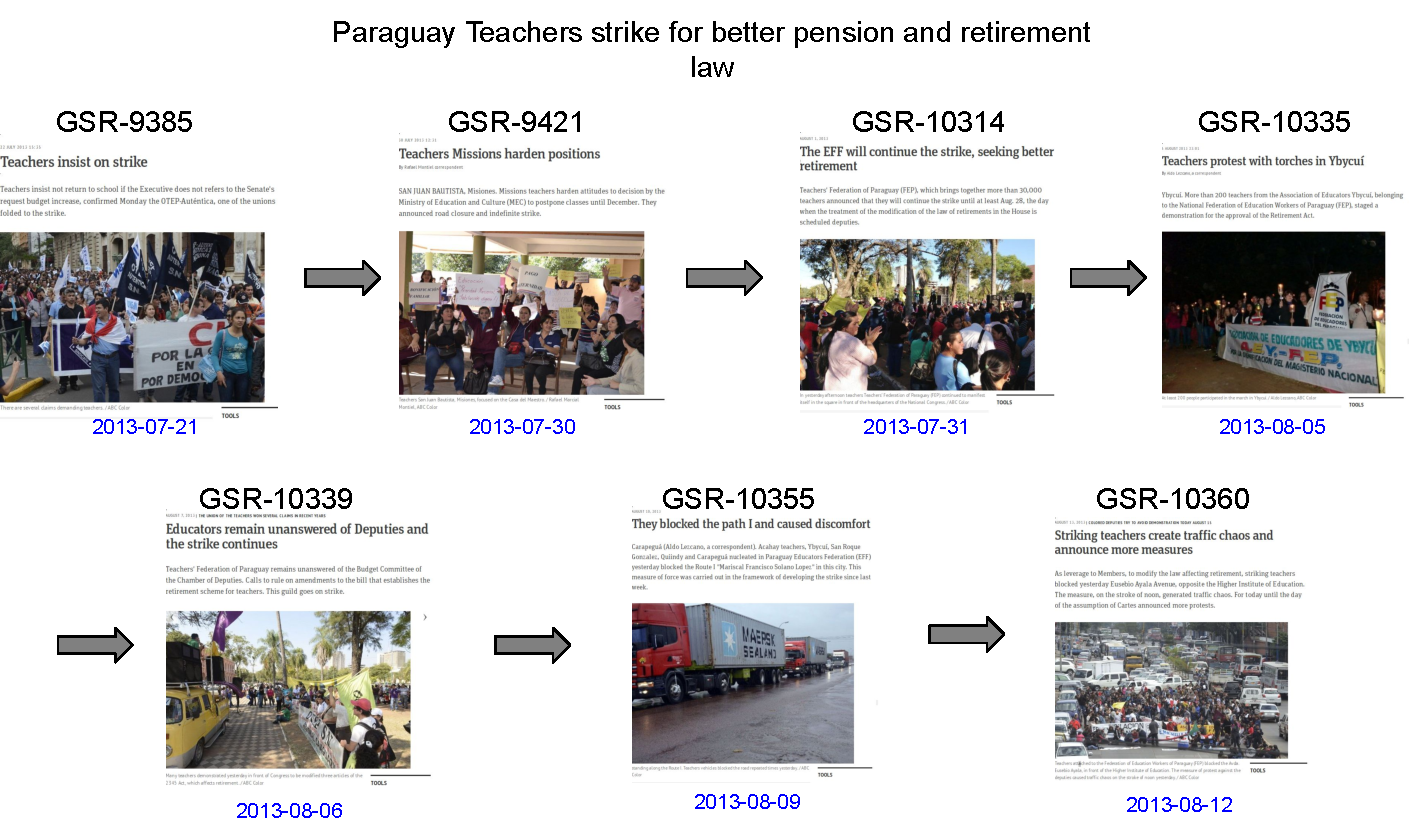
\includegraphics[width=0.9\textwidth]{Problem4/figures/Matching&EventSignificance.pdf}
    \end{figure}
\end{frame}

\begin{frame}
    \begin{itemize}
    \item Understanding of event progressions and grouping helps
    \begin{itemize}
        \item Uncover hidden relations between supposedly unrelated events
        \item Allow an additional dimension of modeling and analysis
        \item identifying uncertain and missing events
    \end{itemize}
    
    \item Possible Approach - Temporal clustering of documents
        \begin{itemize}
                \item Storytelling~\cite{schlachter2015leveraging}
                \item document text is generally not available 
                    \begin{itemize}
                        \item URL's might become invalid over-time
                        \item Example: ICEWS, RavenPack etc
                    \end{itemize}
        \end{itemize}
\end{itemize}
\end{frame}

\begin{frame}{Reasoning over Event Progressions}
    \begin{itemize}
        \item Events can be viewed as Temporal Knowledge Graphs
    \end{itemize}
\begin{figure}
     \centering
     \begin{subfigure}[b]{0.5\textwidth}
         \centering
         \includegraphics[width=0.5\textwidth]{Problem4/figures/know-evolve.png}
         \caption{~\cite{trivedi2017know}}
     \end{subfigure}%
     \hfill
     \begin{subfigure}[b]{0.5\textwidth}
         \centering
         \includegraphics[width=0.8\textwidth]{Problem4/figures/EKG.png}
         \caption{~\cite{gottschalk2018eventkg}}
     \end{subfigure}
\end{figure}
\end{frame}

\section{Proposed Timeline}
\begin{frame}{Proposed Timeline}
\begin{figure}
    \centering
    \includegraphics[width=\textwidth]{Problem4/figures/phdTimeline.pdf}
\end{figure}
\end{frame}